\documentclass[a4paper]{article}

\usepackage[english]{babel}
\usepackage[left=2.5cm,right=2.5cm,top=1cm,bottom=1.5cm]{geometry}
\usepackage[utf8]{inputenc}
\usepackage{amsmath}
\usepackage{amsthm}
\usepackage{amsfonts}
\usepackage{amssymb}
\usepackage{graphicx}
\usepackage{cite}
\usepackage{graphicx}
\usepackage{caption}
\usepackage{subcaption}
\usepackage[colorinlistoftodos]{todonotes}

\usepackage{epsfig}
\usepackage{float}
\usepackage[justification=centering]{caption}

\title{Simulated annealing algorithm for graph coloring}

\author{Xavier Fontaine, Thomas Grivaz, Antoine Mougeot}

\date{\today}

\begin{document}
\maketitle

\begin{abstract}
This report summarizes our methodology and results in the context of experimenting the Markov Chain Monte Carlo method for the problem of graph coloring.
\end{abstract}

\section{Metropolis chain}
\label{sec2}

In this section we run experiments with $\beta$ fixed and we apply the Metropolis-Hastings algorithm as described in the project statement. We analyze the influence of the initial value of $\beta$ on the minimal value of the Hamiltonian reached by our algorithm. We can think of $\beta$ as the inverse of a temperature and therefore we note $T=\dfrac{1}{\beta}$.

In these experiments we fix an Erdös-Renyi graph $G$ with parameters $N=100$ and $c=20$. We use $d=5$ colors. We test three different values of temperature: $T=10$, $T=1$ and $T=0.1$ and we run the simulations with $3000$ iterations. Here are the curves we obtain:

\begin{figure}[H]
 \begin{minipage}[b]{.3\linewidth}
  \centering\epsfig{figure=../Plots/FixedTemperature/courbeT10_I193_F172_M147.png,width=\linewidth}
  \caption{$T=10.0$ and $\min H=147$ \label{fix10}}
 \end{minipage} \hfill
 \begin{minipage}[b]{.3\linewidth}
  \centering\epsfig{figure=../Plots/FixedTemperature/courbeT1_I204_F87_M83.png,width=\linewidth}
  \caption{$T=1.0$ and $\min H=83$ \label{fix1}}
 \end{minipage} \hfill
 \begin{minipage}[b]{.3\linewidth}
  \centering\epsfig{figure=../Plots/FixedTemperature/courbeT01_I215_F50_M50.png,width=\linewidth}
  \caption{$T=0.1$ and $\min H=50$ \label{fix01}}
 \end{minipage}
\end{figure}

\begin{itemize}
\item When $T$ is high (i.e. $\beta$ is small), the probability to accept a move that increases the Hamiltonian is high (for $T=10.0$ it is roughly $80\%$) and consequently the values of $H$ vary a lot. Therefore we observe a lot of fluctuations and the chain does not converge into a precise state. Moreover, the final Hamiltonian value is not equal to the minimal Hamiltonian value. We observe also that since $\beta$ is small, $\pi_{\beta}$ is far away from $\pi_{\infty}$ and then the minimal Hamiltonian value that we reach is really bigger than the global minimum we could reach. With the graph we used and these settings we obtain an average minimal value of $153$ for $H$.
\item With an intermediate value of $T$ ($T=1.0$ here) the previous phenomenon is less visible. The probability to accept a move increasing the Hamiltonian is indeed smaller (about $10\%$ now) and therefore we observe a global decrease of $H$. However we can still see some fluctuations but the final Hamiltonian value is near from the minimal Hamiltonian value reached during the $3000$ iterations. The distribution $\pi_{\beta}$ is still far from $\pi_{\infty}$ and therefore the minimal Hamiltonian value we obtain here (its average is $80$) is still much bigger than the global minimum.
\item When $T$ is low, the probability to increase $H$ is very low and therefore we obtain a function $t \mapsto H(x^t)$ that is non-increasing. Now the distribution $\pi_{\beta}$ is closer to $\pi_{\infty}$ but the probability to get stuck in a local minimum is really high. Therefore the final Hamiltonian value is fast always equal to the minimal Hamiltonian value obtain during the iterations because the chain does not manage to leave this local minimum. However we obtain smaller values for $H$ ($H=50$ in our case on average).
\end{itemize}

Therefore we can conclude that when $T$ is fixed we have to choose a low value for $T$ in order to obtain small values for the Hamiltonian. The drawback of this method is that we are likely to get stuck in a local minimum. However if we increase $T$ we will need too many iterations in order to reach small values of $H$.

In order to obtain better results we will use the method of \textit{Simulated Annealing} which decreases the value of $T$ during the iterations.


\section{Simulated Annealing}
In this section we will describe how we chose and tuned the parameters of our algorithm. In order to minimize the bias we could have regarding the graph we're trying to color, several graphs were considered for each value of a parameter: one random graph with $N=100$, $c=5$ and $q=3$ (which was the graph provided on the project webpage, that we call $G_1$), one random graph with $N=200$, $c=40$, $q=5$ ($G_2$), one random graph with $N=50$, $c=10$, $q=3$ ($G_3$) and finally a random graph with $N=100$, $c=30$, $q=7$ ($G_4$). Besides $G_1$, we chose graphs with high edge probability that result in high final energy after having run the Metropolis algorithm so that's it's easier to notice differences between choices of parameters.

\subsection{Initial Temperature}
According to Kirkpatrick \cite{kirkpatrick}, a suitable temperature $T_0$ is one that results in an average increase of acceptance probability $p_0$ of about 0.8. The value of $T_0$ depends on the scaling of our cost function and hence is problem specific. To estimate this, we conducted an initial search on each graph where all increases are accepted and calculated the average increase over a fixed number of iterations. The initial temperature is given by :
$$T_0=-\dfrac{\mathbb{E}(\Delta_+)}{\mathrm{ln}(p_0)}$$

Where $\Delta_+ = H(x^{new}) - H(x^0)$ is a strictly positive increase. We also tried different base acceptance probabilities (0.5, 0.3) and several fixed values of $T_0$, but this method gave us the best overall results.

\subsection{Cooling Function}
Several ways of decreasing the temperature were considered. We found three cooling functions that gave good results:
\begin{itemize}
\item Exponential schedule: $$T(t)=T_0 \alpha^t$$
We considered $\alpha \in [0.7,0.95]$ and we selected the best value of $\alpha$ with running experiments with a step of $0.01$.
\item Linear schedule: $$T(t)=T_0 -\eta t$$ with $\eta \in [0.05,0.4]$ and a step of $0.05$.
\item Power schedule: $$\forall t \geqslant 1, \ T(t)=\dfrac{T_0}{t^{\gamma}}$$ with $\gamma \in [0,1]$, and a step of $0.1$.
\end{itemize}
Moreover since we did not want to have too low temperatures we chose a minimal value for $T$: $$T(t)=\max(T_{\min},T(t)).$$ We found that $T_{\min}=0.1$ is a good value. 
\\

In order to find the best values for the parameters $\alpha$, $\gamma$ and $\eta$ we ran the Metropolis algorithm on our four graphs with different values for those parameters and we averaged the final energy obtained. We then kept the value for which the final energy was the minimum and ran the whole process again several times to make sure that it was indeed the best overall parameter. Note that even though differences in results were very small (the differences in energy between parameters were in the 5\% range), we noticed that the optimal parameter was consistent from one run to another. We checked also that the parameters we obtained were optimal for each graph taken separately.

Finally we found the following values for our parameters. These are the values that gave the best average results after several runs of the Metropolis-Hastings algorithm.

\begin{center}
\begin{tabular}{|c|c|c|}
\hline 
$\alpha$ & $\eta$ & $\gamma$ \\ 
\hline 
$0.85$ & $0.25$ & $0.5$ \\ 
\hline 
\end{tabular} 
\end{center}

\subsection{Epoch length}

We found out that decreasing the temperature at each iteration was not the best cooling scheme. Indeed when $T$ is low, the probability to accept increasing moves is small and therefore we need to stay at the same value of the temperature before accepting some moves. If we decrease directly the value of $T$ we do not really take profit of the effect of intermediate temperature values. That is why we tried to decrease the temperature every $x$ iterations, where $x \geqslant 2$ is an integer to find. In order to find this epoch length we run the Metropolis algorithm several times with different values of $x$ and we chose the value of $x$ that gave the best average results. We also set the number of iterations to $10,000$ to make sure to reach convergence.We summarize our results in the following tabular:
\begin{center}
\begin{tabular}{| c || c | c| c| c| c|}
\hline
Epoch & 1 & 2 & 3 & 5 & 10\\
\hline
Average minimum Hamiltonian & 131.17 & 126.77 & 126.98 & 124.67 & 127.59\\
\hline
\end{tabular}
\captionof{table}{Epoch length results}
\end{center}

We find that an epoch of $5$ gives good results. However, as we said it, for low temperatures the acceptance probability of moves that increase the Hamiltonian is low and therefore we have to stay at the same temperature during few iterations to see the effect of this temperature value. This remark suggests to try non-constant epoch lengths, i.e. to wait longer times before decreasing the temperature when $T$ is low.

A possible scheme to implement this is the following:
\begin{equation*}
\left\{
\begin{aligned}
&\textrm{if }T>5, \textrm{ decrease temperature every 5 iterations}\\
&\textrm{if }T>1, \textrm{ decrease temperature every 10 iterations}\\
&\textrm{if }T>0.1, \textrm{ decrease temperature every 20 iterations}\\
\end{aligned}
\right.
\end{equation*}

\subsection{Determination of the best decreasing function}

In order to choose the best decreasing function, we plot on the same graph the average curves obtained for the three cooling schemes presented above. In order to decrease the bias due to randomness we work on fixed graphs with the same initial random coloring and we average the results on $10$ runs.

Here are the curves $(t \mapsto H(x^t))$ for the three schemes. 
\begin{figure}[H]
    \centering
    \begin{subfigure}[b]{0.45\textwidth}
        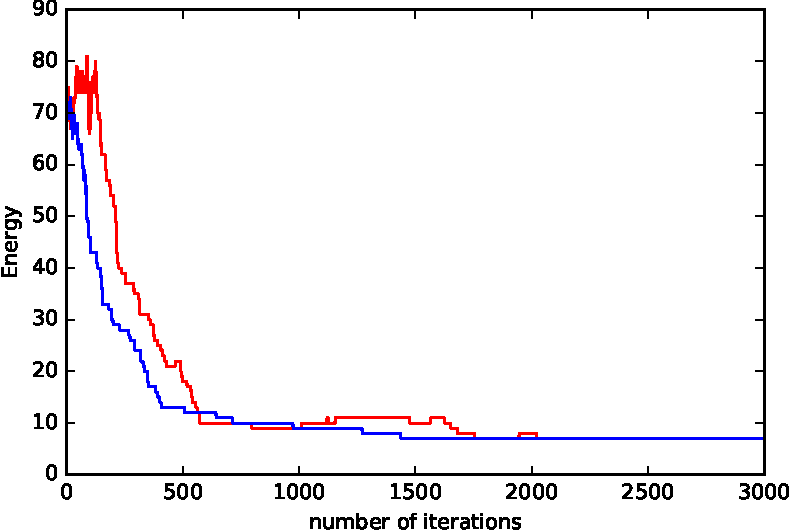
\includegraphics[width=2.3in, height = 1.7in]{H_G1_cropped.pdf}
        \caption{$G_1$}
        \label{fig:g1}
    \end{subfigure}
    ~ %add desired spacing between images, e. g. ~, \quad, \qquad, \hfill etc. 
      %(or a blank line to force the subfigure onto a new line)
    \begin{subfigure}[b]{0.45\textwidth}
        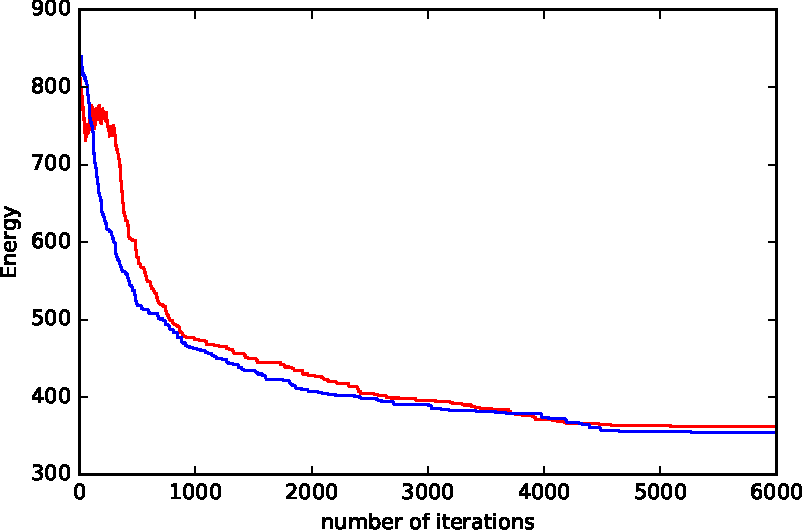
\includegraphics[width=2.3in, height=1.7in]{H_G2_cropped.pdf}
        \caption{$G_2$}
        \label{fig:g2}
    \end{subfigure}
    ~ %add desired spacing between images, e. g. ~, \quad, \qquad, \hfill etc. 
    %(or a blank line to force the subfigure onto a new line)
    
    \begin{subfigure}[b]{0.45\textwidth}
        \centering\epsfig{figure=../Plots/SimulatedAnnealing/G3_275_267_259.png,width=\linewidth}
        \caption{$G_3$}
        \label{fig:g3}
    \end{subfigure}
    ~ %add desired spacing between images, e. g. ~, \quad, \qquad, \hfill etc. 
      %(or a blank line to force the subfigure onto a new line)
    \begin{subfigure}[b]{0.45\textwidth}
        \centering\epsfig{figure=../Plots/SimulatedAnnealing/G4_464_465_48.png,width=\linewidth}
        \caption{$G_4$}
        \label{fig:g4}
    \end{subfigure}
    ~ %add desired spacing between images, e. g. ~, \quad, \qquad, \hfill etc. 
    %(or a blank line to force the subfigure onto a new line)
    \caption{Evolution of the energy of the Metropolis algorithm for two graphs. The blue curve corresponds to a linear scheme, the green one to an exponential scheme while the red curve represents the evolution of the energy using a power scheme.}
    \label{fig:comparison}
\end{figure}

As we can see from figure \ref{fig:comparison}, results are pretty similar. We choose the power decrease scheme because it seems to give the best results. However, there is still some variance in the results and other cooling models can also give good results.

\subsection{Utility of Simulated Annealing}

In this subsection we want to compare the results obtained with simulated annealing and the results obtained in section \ref{sec2} without simulated annealing. Therefore we run experiments on the same graph as in section \ref{sec2} with the decreasing function described in the previous part. We obtain the following results (the minimal Hamitonian value is computed as an average on $10$ runs):

\begin{figure}[H]
 \begin{minipage}[b]{.45\linewidth}
  \centering\epsfig{figure=../Plots/SimulatedAnnealing/courbe_mygraph_45.png,width=\linewidth}
  \caption{Simulated annealing gives $\min H=47$ \label{sim}}
 \end{minipage} \hfill
 \begin{minipage}[b]{.45\linewidth}
  \centering\epsfig{figure=../Plots/FixedTemperature/courbeT01_I215_F50_M50.png,width=\linewidth}
  \caption{$T=0.1$ gives $\min H=50$ \label{fix01bis}}
 \end{minipage}
\end{figure}


As we can see on the figure, we obtain better results with simulated annealing and a minimal temperature around $0.1$ than with setting directly the temperature to $0.1$ and keeping it fixed. This justifies the use of simulated annealing to obtain better results.

\subsection{Influence of Graph density $c$ on $H_{\min}$}

We plot the curve $H_{\min}$ as a function of $c$ for some fixed values of $q$ and $N=100$. The value of $H_{\min}$ is obtained by computing the average value of the minimum Hamiltonian for several Erdös-Renyi graphs with the same parameters. We obtain the following curves.

\begin{figure}[H]
 \begin{minipage}[b]{\linewidth}
  \centering\epsfig{figure=../Plots/Hmin/hmin_quick.png,width=0.5\linewidth}
  \caption{$H_{\min}$ as a function of $c$ (blue: $q=3$, green: $q=5$, red: $q=7$) \label{hmin}}
 \end{minipage}
\end{figure}

We observe two phenomenas:
\begin{enumerate}
\item $H_{\min}$ is a decreasing function of $q$. This is conform to our intuition because if we have more colors to color a graph, it is easier to color it properly or to have a small Hamiltonian value.
\item There seems to be a phase transition in the behavior of the graph regarding its colorability. There is a threshold value $c_{\mathrm{th}}(q)$ such that for $c<c_{\mathrm{th}}(q)$, the graph is colorable with our algorithm and for $c>c_{\mathrm{th}}(q)$, the graph is not colorable with our algorithm. However saying that our algorithm is not able to color the graph does not mean that there is no proper coloration of the graph but only that it is too difficult to find for our algorithm. Besides we can suppose that there exists another threshold value for $c$ concerning the colorability of the graph, which will be above $c_{\mathrm{th}}(q)$. As remarked in the first point, $H_{\min}$ is a decreasing function of $q$ and therefore $c_{\mathrm{th}}(q)$ is an increasing function of $q$. Moreover the phase transition is very easy to observe on the graph because the slope of the curve seems to be affine by steps and the slope of the second part of the curve is really bigger than the slope of the first part.
\end{enumerate}

\bibliography{bibli_RW}
\bibliographystyle{plain}
\end{document}